
\documentclass[letterpaper,12pt]{article}

\usepackage{graphics,graphicx}
\usepackage{aas_macros}

\usepackage[svgnames]{xcolor}
\definecolor{darkgrey}{RGB}{83, 92, 104}

\usepackage[font={color=ocre,bf}]{caption}
\usepackage{subcaption}
\usepackage{cancel}
\usepackage{wrapfig}

\usepackage{fontspec}
\usepackage[T1]{fontenc}
\usepackage{newtxsf}
\setmainfont{Fira Sans Book}[Scale=0.95]


\usepackage[backref,breaklinks,colorlinks,urlcolor=blue,citecolor=blue,linkcolor=blue]{hyperref}
\bibliographystyle{plain}
\usepackage{cleveref}

%%%%%%%%%%%%%%%%%%%%%%%%%%%
%%%%% Page dimensions %%%%%
%%%%%%%%%%%%%%%%%%%%%%%%%%%

\setlength{\textwidth}{6.5in}
\setlength{\textheight}{9in}
\setlength{\topmargin}{-0.0625in}
\setlength{\oddsidemargin}{0in}
\setlength{\evensidemargin}{0in}
\setlength{\headheight}{0in}
\setlength{\headsep}{0in}
\setlength{\hoffset}{0in}
\setlength{\voffset}{0in}



%%%%%%%%%%%%%%%%%%%%%%%%%%%%%%%%%%
%%%%% Section heading format %%%%%
%%%%%%%%%%%%%%%%%%%%%%%%%%%%%%%%%%

\makeatletter
\renewcommand{\section}{\@startsection%
{section}{1}{0mm}{-\baselineskip}%
{0.5\baselineskip}{\normalfont\Large\bfseries}}%
\makeatother

%%%%%%%%%%%%%%%%%%%%%%%%%%%%%%%%%%%%%
%%%%% Some Useful Abbreviations %%%%%
%%%%%%%%%%%%%%%%%%%%%%%%%%%%%%%%%%%%%
\newcommand{\tess}{{\it TESS}}
\newcommand{\jwst}{{\it JWST}}
\newcommand{\kepler}{{\it Kepler}}
\newcommand{\ktwo}{{\it K2}}
\newcommand{\hst}{{\it HST}}
\newcommand{\msun}{$M_{\odot}$}
\newcommand{\rsun}{$R_{\odot}$}
\newcommand{\lsun}{$L_{\odot}$}
\newcommand{\re}{$R_{\oplus}$}
\newcommand{\me}{$M_{\oplus}$}
\newcommand{\rj}{$R_{\textrm{\scriptsize Jup}}$}
\newcommand{\mj}{$M_{\textrm{\scriptsize Jup}}$}
\newcommand{\ms}{m~s$^{-1}$}

%%%%%%%%%%%%%%%%%%%%%%%%%%%%%
%%%%% Start of document %%%%%
%%%%%%%%%%%%%%%%%%%%%%%%%%%%%

\begin{document}
\pagestyle{plain}
\pagenumbering{arabic}


%%%%%%%%%%%%%%%%%%%%%%%%%%%%%
%%%%% Title of proposal %%%%%
%%%%%%%%%%%%%%%%%%%%%%%%%%%%%

\begin{center}
\bfseries\uppercase{%
%%
%% ENTER TITLE OF PROPOSAL BELOW THIS LINE
Mitigating exoplanet radius biases from wavelength dependence of starspot contrast
%%
%%
}
\end{center}


%%%%%%%%%%%%%%%%%%%%%%%%%%%%%%%%%%%%%%%%%
%%%%% Body of science justification %%%%%
%%%%% and technical feasibility     %%%%%
%%%%%%%%%%%%%%%%%%%%%%%%%%%%%%%%%%%%%%%%%

Starspots bias percieved exoplanet radii \cite{2018ApJ...853..122R}.  Here we propose a systematic approach to quantify and mitigate starspot-induced exoplanet radius biases based on a large sample of spotted stars to be observed in \tess\ Cycle 4.  The approach will deliver constraints on both the typical starspot coverage fraction and the typical starspot temperature contrast, as a function of spectral type and rotation rate.  This mapping can then serve as a ``lookup table'' for practitioners to gauge the extent to which a given source is likely to suffer from starspot-induced exoplanet radius biases.  No such reliable lookup table presently exists for main sequence stars, owing to the inability of differential lightcurves to account for \emph{total} starspot coverage fractions \cite{2018ApJ...865..142B}.  This program will leverage the significant overlap of the \tess\ Cycle 4 fields with the \ktwo\ fields.

\section{Scientific Justification: The Transit Light Source Effect}
The diminution of flux arising from occultations of the stellar disk contains information the relative sizes of the occulting bodies.  A commonsense exoplanet heuristic dictates that the relative transit depth $D$ equals the ratio of the bodies' projected areas ($R_p^2/R_\star^2$).  Additional correction factors account for limb darkening \cite{2002ApJ...580L.171M}.  Starspots on a stellar surface can exhibit spatial segregations
that yield \emph{unocculted starspots}: spots that are present on the surface but are not traversed during transits.  These unocculted starspots confound the mapping of transit depth to planet radius: a planet ``looks bigger'' than it really is if it blocks the brighter-on-average flux of the stellar disk \cite{2018AJ....156...91M}.  \textbf{You cannot measure a planet radius without making some assumptions about the extent, contrast, and distribution of starspots.}

The prevailing assumption within the exoplanet community has been that starspot covering fractions are small enough---as in Sunspots---to be ignored.  New theoretical models \cite{2018ApJ...853..122R} and observational evidence \cite{2016MNRAS.463.2494F} indicate that starspot covering fractions are large enough to bias transit depths beyond the level of precision of \kepler\ and \tess.  This so-called ``Transit Light Source Effect'' (TLSE) can bias derived exoplanet radii up to 17\% in the \tess\ bandpass, and can bias derived exoplanet \emph{densities} up to 50\%, since the radius error propagates into volume error with a factor of 3.  Therefore, TLSE threatens placement and interpretation of the exoplanet mass-radius relation science requirements of the \tess\ mission.  The interpretation of \jwst\ exoplanet transmission spectroscopy is also at risk \cite{2019AJ....157...11W}.

\section{Analysis Plan: Compare \tess\ and \ktwo\ amplitudes}

\noindent\textbf{Kepler and TESS perceive different starspot contrasts.}

Starspots emit light, which is often parameterized as \emph{spot contrast}, $c$, where $0$ means the spots are completely black compared to the bright photosphere, and $c=0.3$ means the spot has 30\% the flux per-unit-surface-area of the pristine photosphere.  Hypothetically, a contrast of unity would mean the starspot blends into ambient photosphere, its border vanishing entirely.  Spot contrast is wavelength dependent ($c_\lambda$). It has a spectrum of its own, starting close to zero in the blue/visible, and approaching perhaps 40\% in the near-IR; the exact prescription remains an active research area \cite{2005LRSP....2....8B}.  Zeeman splitting and other magnetic phenomena are secondary to the mere fact that starspots appear as cooler-than-average regions on the stellar surface.  

Starspot flux can be parameterized by labeling the emission components with a characteristic temperatures $T_\text{spot}<T_\text{phot}$.  The spot and ambient photosphere spectra depend only on those temperatures: $S(T_\text{spot})$ and $S(T_\text{phot})$.  The wavelength-dependent spot contrast is then simply the ratio of the spot spectrum to the ambient photosphere spectrum:  $c_\lambda = \frac{S(T_\text{spot})}{ S(T_\text{phot})}$.

\captionsetup[figure]{font={color=darkgrey,md},textfont={small,singlespacing,md},labelfont={bf,normalsize,color=Black},labelformat={simple},labelsep=period,name={Figure}}



\begin{figure}[hbt!]
    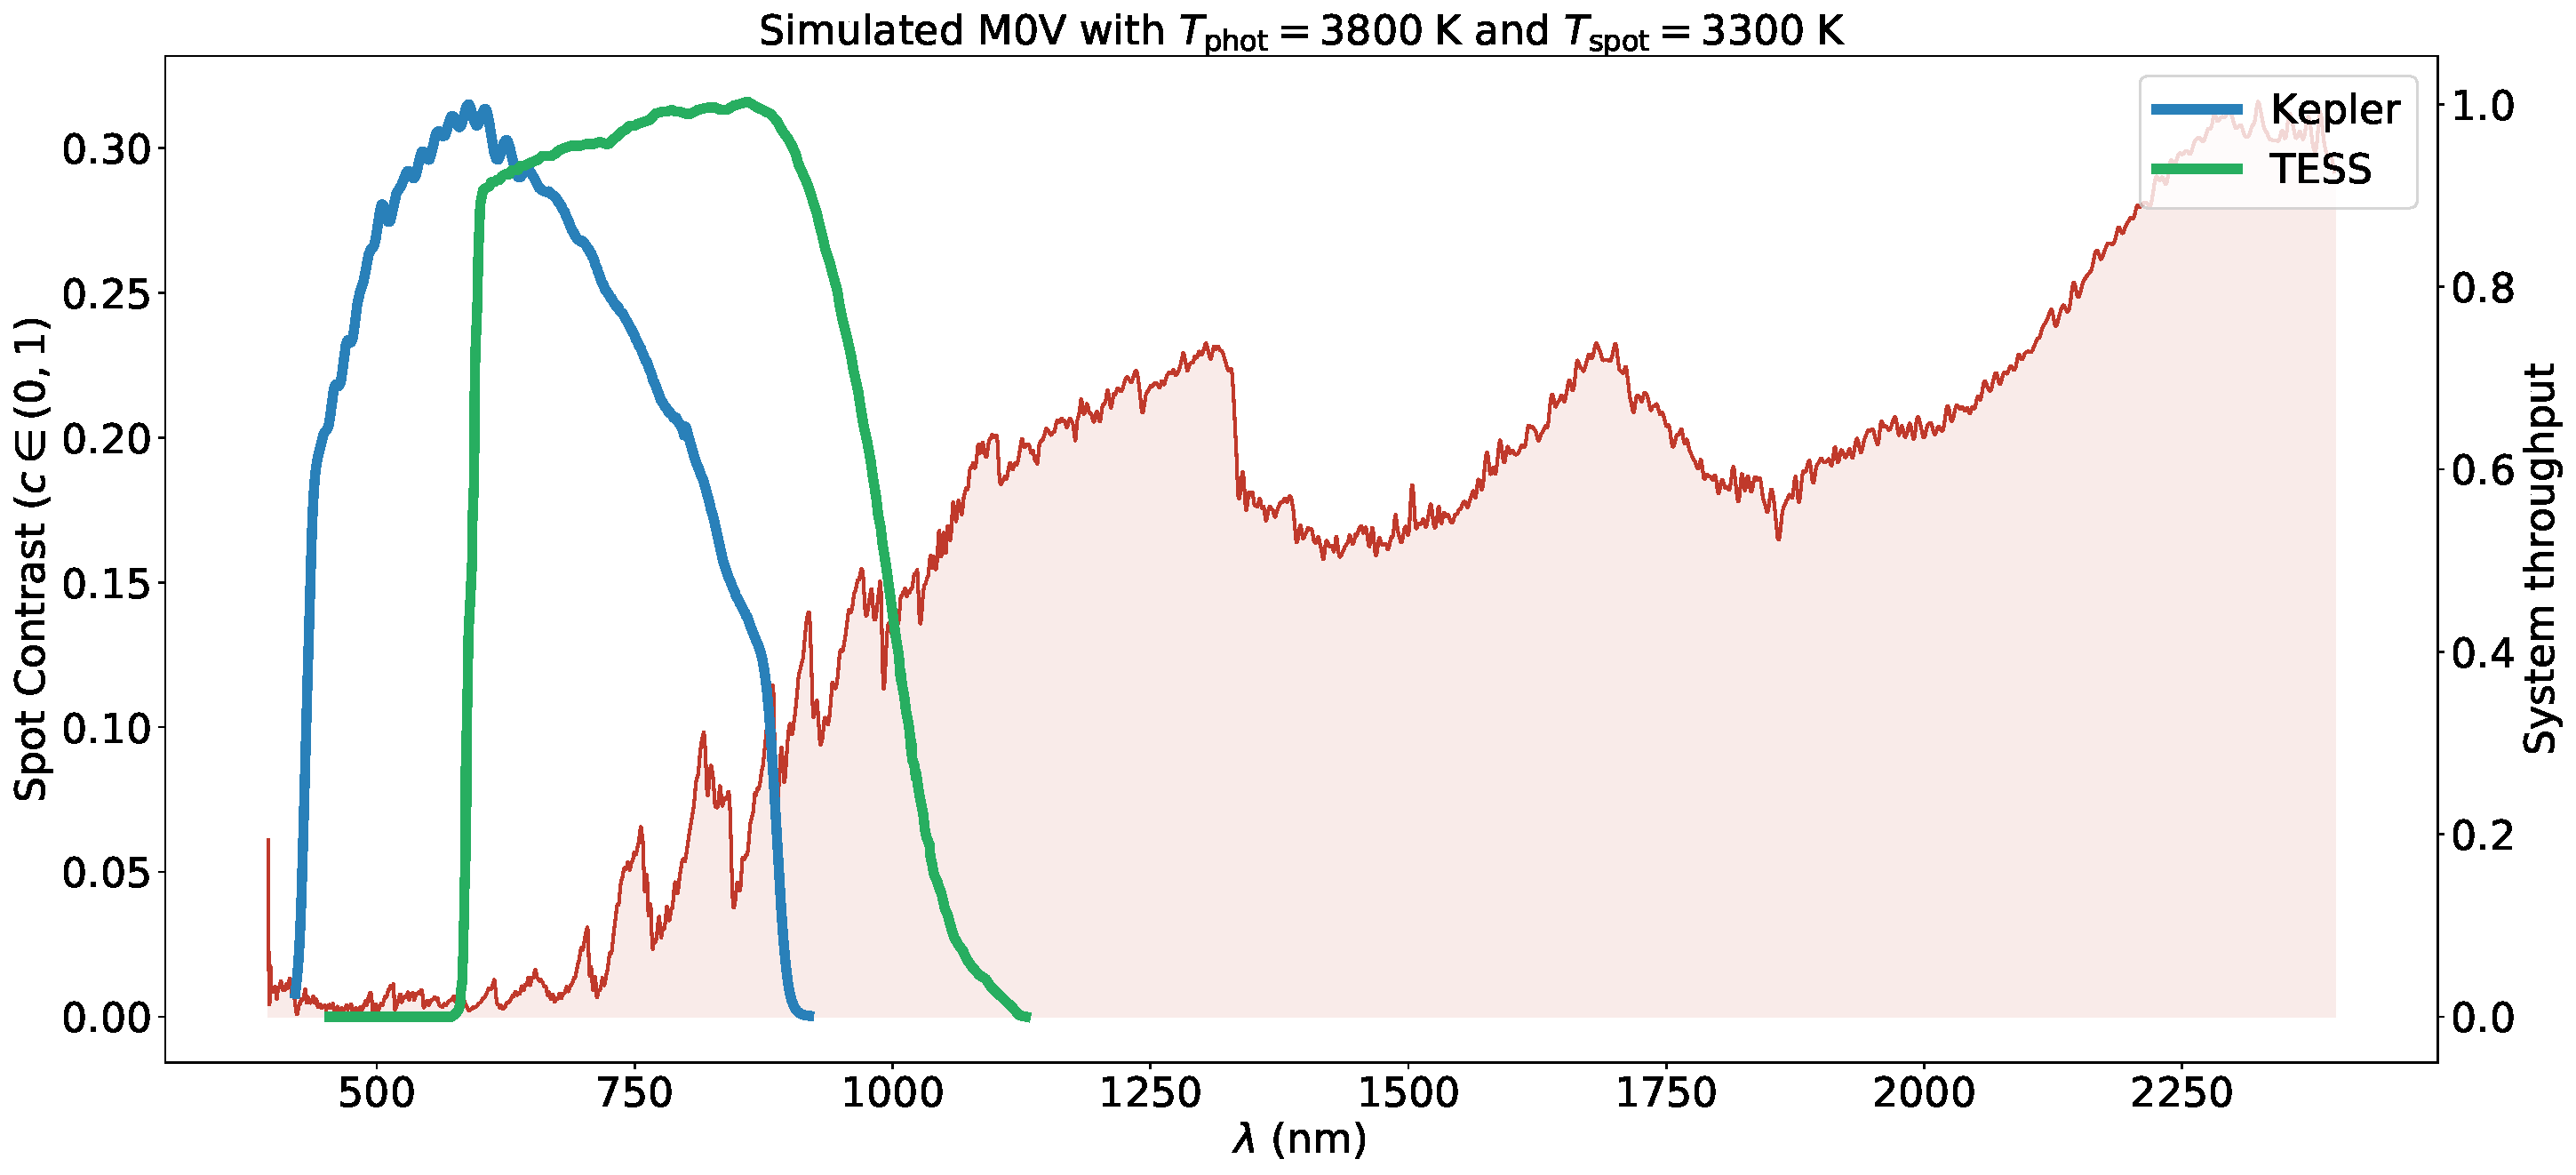
\includegraphics[width=0.95\textwidth]{figures/contrast_spectrum.pdf}
    \caption{Illustration of starspot contrast as seen in \tess\ and \kepler. The red shaded spectrum illustrates the contrast for an M0V spectral type for a choice of spot and ambient photospheric temperatures. The thick blue left-most curve illustrates the \kepler\ passband, the thick green line to its right illustrates the \tess\ passband centered near 850 nm.  A lower number means darker spots.  }
    \label{fig:filtercurve}
\end{figure}

Figure \ref{fig:filtercurve} shows an illustration of wavelength dependent spot contrast for a hypothetical M0V star with $T_\text{phot}=3800\;$K, and with $T_\text{spot}=3300\;$K.  We employ \texttt{PHOENIX} synthetic spectral models \cite{2013A&A...553A...6H}, accessed at these temperatures.  The contrast ascends from near 0.01 at $\lambda=500\;$nm, to 0.15 at 1 $\mu$m.  By 2.3 $\mu$m, the contrast has peaked at 0.3.  The overlapping \kepler\ and \tess\ system throughputs overplotted on Figure \ref{fig:filtercurve} indicate that---on average---the starspot contrast is a lower number in the \kepler passband ($\lambda \sim 550\;$nm)  than for the redder \tess passband ($\lambda \sim 850\;$nm).  Starspots look blacker in \kepler\ and \ktwo\ than they do in \tess.  The understanding of wavelength dependent starspot contrast is not novel--- it has driven the design of precision radial velocity (PRV) spectrographs to the near-IR, where the deleterious effect of starspots on RV jitter is lessened.  \textbf{The key innovation of this proposal stems from the vast number of sources with existing \ktwo\ data that \tess\ will observe in Cycle 4.  This proposal aims to quantify precisely the starspot contrast differences between the \tess\ and \kepler\ wavelength bands.}  We re-iterate that the extent to which nature produces starspot spectra resembling the prescription in Figure \ref{fig:filtercurve} remains an unknown, and is the main thrust of the proposed work effort.  

System-throughput-weighted contrast spectra can be integrated over the illustrated filter curves to yield precision estimates for contrasts in the two passbands.  For this M0V example, we obtain $c_{\ktwo}\sim0.025$ and $c_{\tess}\sim0.1$.  Starspots appear about four times darker in \kepler\ and \ktwo\ than they do in \tess.  We define the ratio of starspot contrasts of \tess\ compared to \kepler\ as $\mathcal{R}\equiv \frac{c_{\tess}}{c_{\ktwo}}$.  This proposal will systematically measure $\mathcal{R}$ for a vast number of stars observed by both missions.
\newline


\noindent \textbf{Spot-induced modulation amplitudes depend on contrast.}  

Rotationally-modulated lightcurves exhibit semi-sinusoidal undulations as starspots (or spot groups) enter and exit the projected stellar disk.  The most-spotted projected hemisphere is directed towards the observer at the moment of the lightcurve minimum, and the least-spotted projected hemisphere at lightcurve maximum.  The amplitude of the lightcurve, therefore, is approximately the difference in starspot coverage fractions $\Delta f_{spot} \equiv f_{max}-f_{min}$ between the most-and-least spotted projected hemispheres, weighted by the spot contrast: $ A_\lambda = \Delta f_{spot} \cdot (1-c_\lambda)$.  Therefore the ratio of \tess\ to \kepler\ amplitudes yields a constraint independent of the actual spot coverage fraction:

$$ \frac{A_{TESS}}{A_{Kepler}} = \cancel{\frac{\Delta f_{spot}}{\Delta f_{spot}}} \cdot \frac{1-c_{TESS}}{1-c_{Kepler}} $$

The notation is cumbersome, but the takeaway is clear: \textbf{we can quantify spot contrast ratio knowing only the amplitudes of \ktwo\ and \tess\ spot-modulated lightcurves.}  This equation is approximate, and in practice our team will derive $\mathcal{R}= \frac{c_{\tess}}{c_{\ktwo}}$ with Monte Carlo methods to take into account the uncertainty of the amplitude determination and subtle starspot self-dilution effects.
\newline

\noindent \textbf{Head-to-head comparison of K2 and TESS amplitudes in the ecliptic fields}

\begin{wrapfigure}[23]{r}[10pt]{2.6in}
    \vspace{0mm}
    \begin{center}
    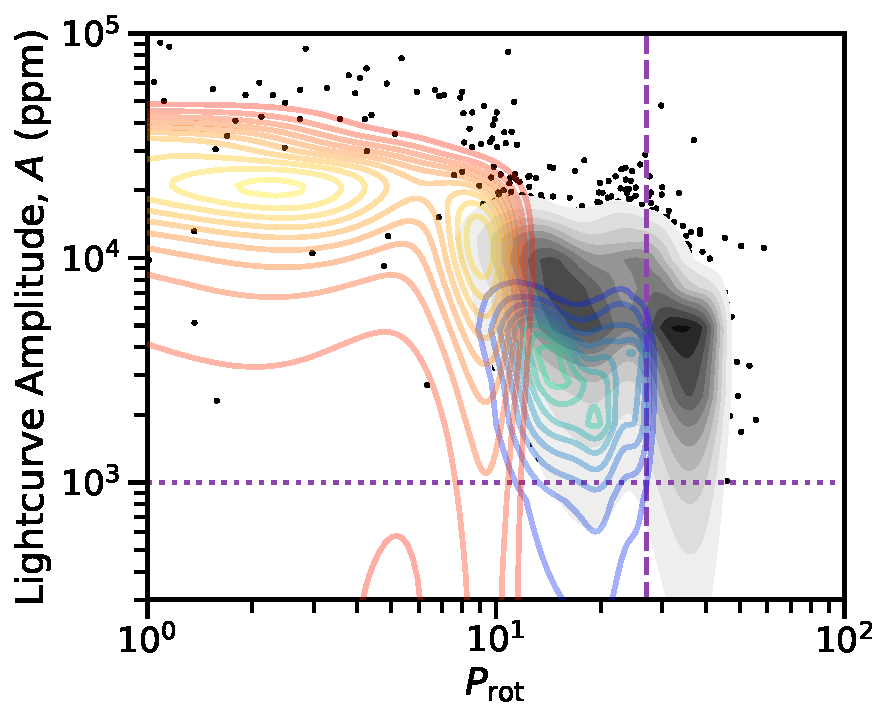
\includegraphics[width=2.6in]{figures/fig1.pdf}
    \caption{Expected signal strength of starspot contrast for the same stars measured in \tess\ and \kepler. }
    \label{fig:expected}
    \vspace{0mm}
\end{center}
\end{wrapfigure}


Ideally, we would have simultaneously observed the same targets with \ktwo\ and \tess\ to measure the instantaneous amplitudes for individual stars.  Cycle 4 provides a unique opportunity to compare the amplitudes of \tess\ and \ktwo\ for the largest sample to date.

The main two factors that affect spot-modulation lightcurve amplitudes are effective temperature (\emph{i.e.} mass), and rotation period (\emph{i.e.} stellar activity/magnetic fields) \cite{2014ApJS..211...24M}.  Other important-albeit-unknown factors like stellar inclination angle and multiplicity \emph{cancel out} when we compare the same stars head-to-head.  We, therefore, propose to follow \cite{2014ApJS..211...24M} by constructing plots of amplitude versus period, subdivided into bins of effective temperature.  The two samples should look identical in these plots, but the locus of \tess\ sources is expected to fall below the \kepler\ sample, as in Figure \ref{fig:expected}.


\tess\ Cycle 4 will observe XX sources in the \ktwo\ campaign fields.  The fact that observations are not contemporaneous adds some \emph{cosmic variance}: stars wander into and out-of their respective stellar minimum and maximum activity cycles. On average stars will enter and exit stellar activity cycles in equal measure, injecting per-star variance, but keeping the subsample mean amplitudes the same.

\section{Technical Feasibility: Consistency is key}

Measuring periods and amplitudes of \kepler\ and \tess\ lightcurves is a routine operation, with relatively low risk.  

The yield of spotted stars in \tess\ will number in the hundreds of thousands.  The \tess\ and \ktwo\ missions both target cool main sequence stars with an abundance of K and M dwarfs.  This program will focus on the rapidly rotating stars ($P_{rot}<20$ days), which exhibit relatively large amplitudes ($A>2000$ ppm), illustrated in panel D of Figure \ref{fig:predictAmps}.  This program will attempt---on a best effort basis---to measure slower rotating stars with ($P_{rot}<20$ days), which have periods comparable to typical observation windows of 27$-$54 days, and amplitudes comparable to the precision limits of \tess.

\section{Expected Impact}

The main deliverable of this work will be a probabilistic assessment of the starspot temperature and starspot coverage faction for every star with a measured starspot modulation period and amplitude in \tess.  These probability distributions will empower exoplanet researchers to correct for biases in exoplanet transit radii.  The probability distributions will reflect all the available information garnered from \tess\ and reasonable assumptions about starspot geometrical distributions.

The starspot properties are also of intrinsic astrophysical interest.  Trends in $T_{spot}$ with rotation rate and mass can reveal important clues to stellar activity, magnetic fields, and stellar atmospheres.  This work will directly address starspot-induced scatter and bias in isochronal-derived stellar ages \cite{2015ApJ...807..174S, 2017ApJ...836..200G}.




\section{Work Plan}

PI will carry out the data analysis using custom scripts that build upon the heritage of the \ktwo\ data analysis ecosystem, including \texttt{lightkurve} and \texttt{celerite}.  The PI will first apply these scripts to \ktwo\ lightcurves.  Undergraduate and graduate students will lead the application of TESS-adapted scripts to \tess\ FFI lightcurves with \texttt{TESS-cut} and \texttt{elenor}.  Half of the funding will go to 1 undergraduate and 1 graduate student Summer 2020 salary, and 0.3 FTE to support the PI.  All reproducible scripts---including Jupyter Notebook tutorials---will be publicly available and developed openly on GitHub.
PI will provide students with an interactive tool to visualize periodic lightcurve structures to aid rapid visual spot-checking of the multidimensional analysis output.  Finally, a High-Level Science Product (HLSP) will be delivered to MAST that contains the following information for each star found to possess detectable starspot-induced lightcurve modulation: 1) the period or periods, 2) an iteratively determined outlier mask of stellar flares, occultations, or spurious data artifacts, 3) a background-star amplitude-dilution estimate, 4) a probability distribution for the spot temperature and coverage fraction, 5) addition model fitting metadata.  PI will co-advise---with Co-I---students in the writeup of the paper(s), authored and/or coauthored by students.


\newpage

\bibliography{tessgi_gully_cycle4}


\end{document}
